\documentclass{article}
\usepackage{ifpdf}
\usepackage[no-math]{fontspec}
%\usepackage[T1]{fontenc}
\usepackage[utf8]{inputenc}
\usepackage[english]{babel}
\usepackage{graphicx}
\usepackage{listings}
\setmainfont[Ligatures=TeX]{Palatino Linotype}

\title{Automaton 0x02}
\author{David E. Shere}

\begin{document}
\maketitle

The phenomenon of \textit{cellular automata} is a well studied topic in mathematics that can be used to model interactions between discrete ``cells'' in a number of disciplines.
In physics the concept has been used in the creation of theoretical models of reality, in which the universe is conceived of as composed of individual cells effected by their neighbors.
Gas and fluid dynamics, too, can be modeled using this concept, leading to simulations that can be used to study the interactions of particles.
My automata sculptures embody the concept by producing and displaying the interactions of cells.
It is conceptually important that the sculptures not be a predetermined set of states, but be the natural product of the interaction of the individual cells.
By creating individual cells in communication with each other, my sculptures become authentic and aesthetic monuments to the beauty and importance of this phenomenon.

With \textit{Automaton 0x02} I have rethought my method of implementation for this series of works.
In \textit{Automaton 0x00} and \textit{Automaton 0x01} the cells were "virtual" cells, all emulated in software on a single microcontroller.
This microcontroller would then calculate the next state in its entirety before telling all the lights that represented cells to turn on or off.
For this new work I have moved from an emulation of cells to an actual hardware implementation of concept.
I have designed a development board for these sculptures that allow the arbitrary connection of cells to each other, producing a network of cells controller by their neighbors they are physically connected to.

For \textit{Automaton 0x02} I have not fully taken advantage of the possibilities, but it is a proof of concept for the utility of this new method for programming \textit{Automata} series sculptures.
Because the cells of automata created with these boards are ruled by their physical connections, new arrangements can be created by simply creating new or removing old connections.
This opens up the possibility for physical control of the set of cells while the sculpture is running and therefore the possibility of interactive installations with them.
Although possible with my old implementation, the distributed nature of this new method also makes the possibility of room sized installation more feasible.
Once again, the distributed nature of this implementation allows cells to only need connections to their actual neighboring cells, rather than running wires from a single "brain" to each cell.

\lstinputlisting[language=c, caption="MSP430 Firmware", frame=L]{main.c}

\begin{figure}[p]
    \centering
    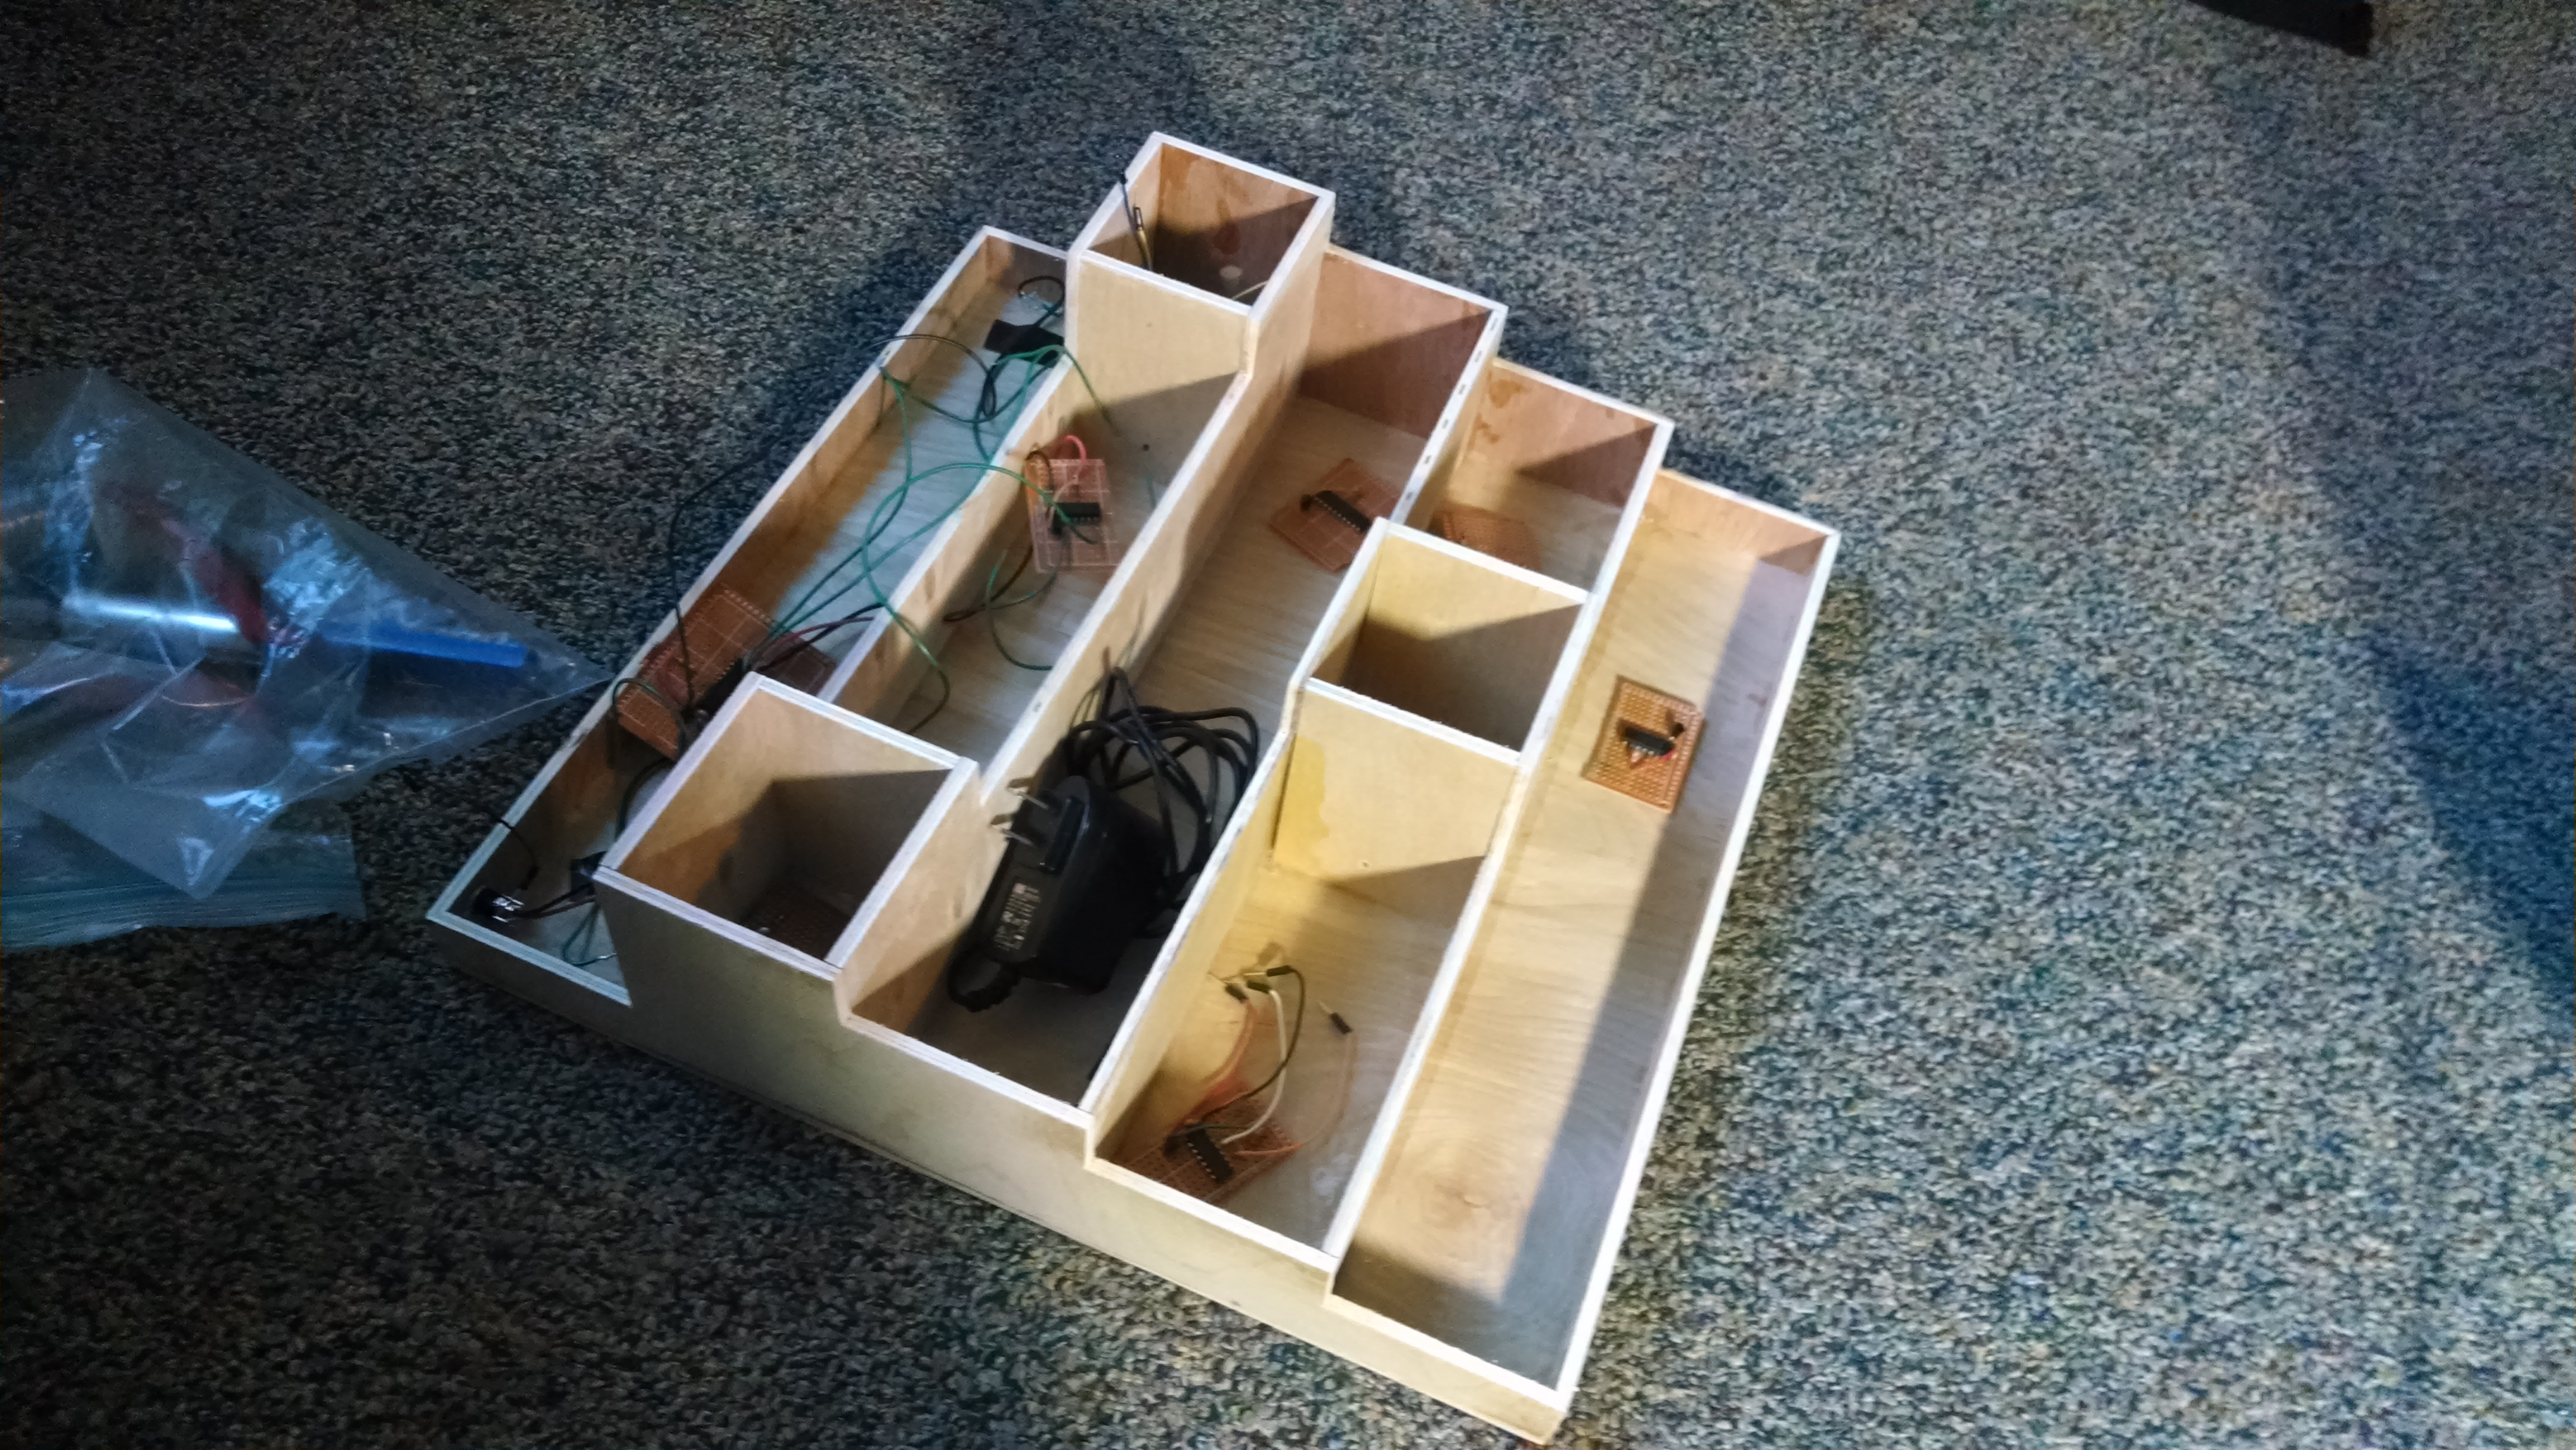
\includegraphics[width=1\textwidth]{sculpture-wip.jpg}
    \caption{Sculpture in development.}
    \label{fig:wip}
\end{figure}

\begin{figure}[p]
    \centering
    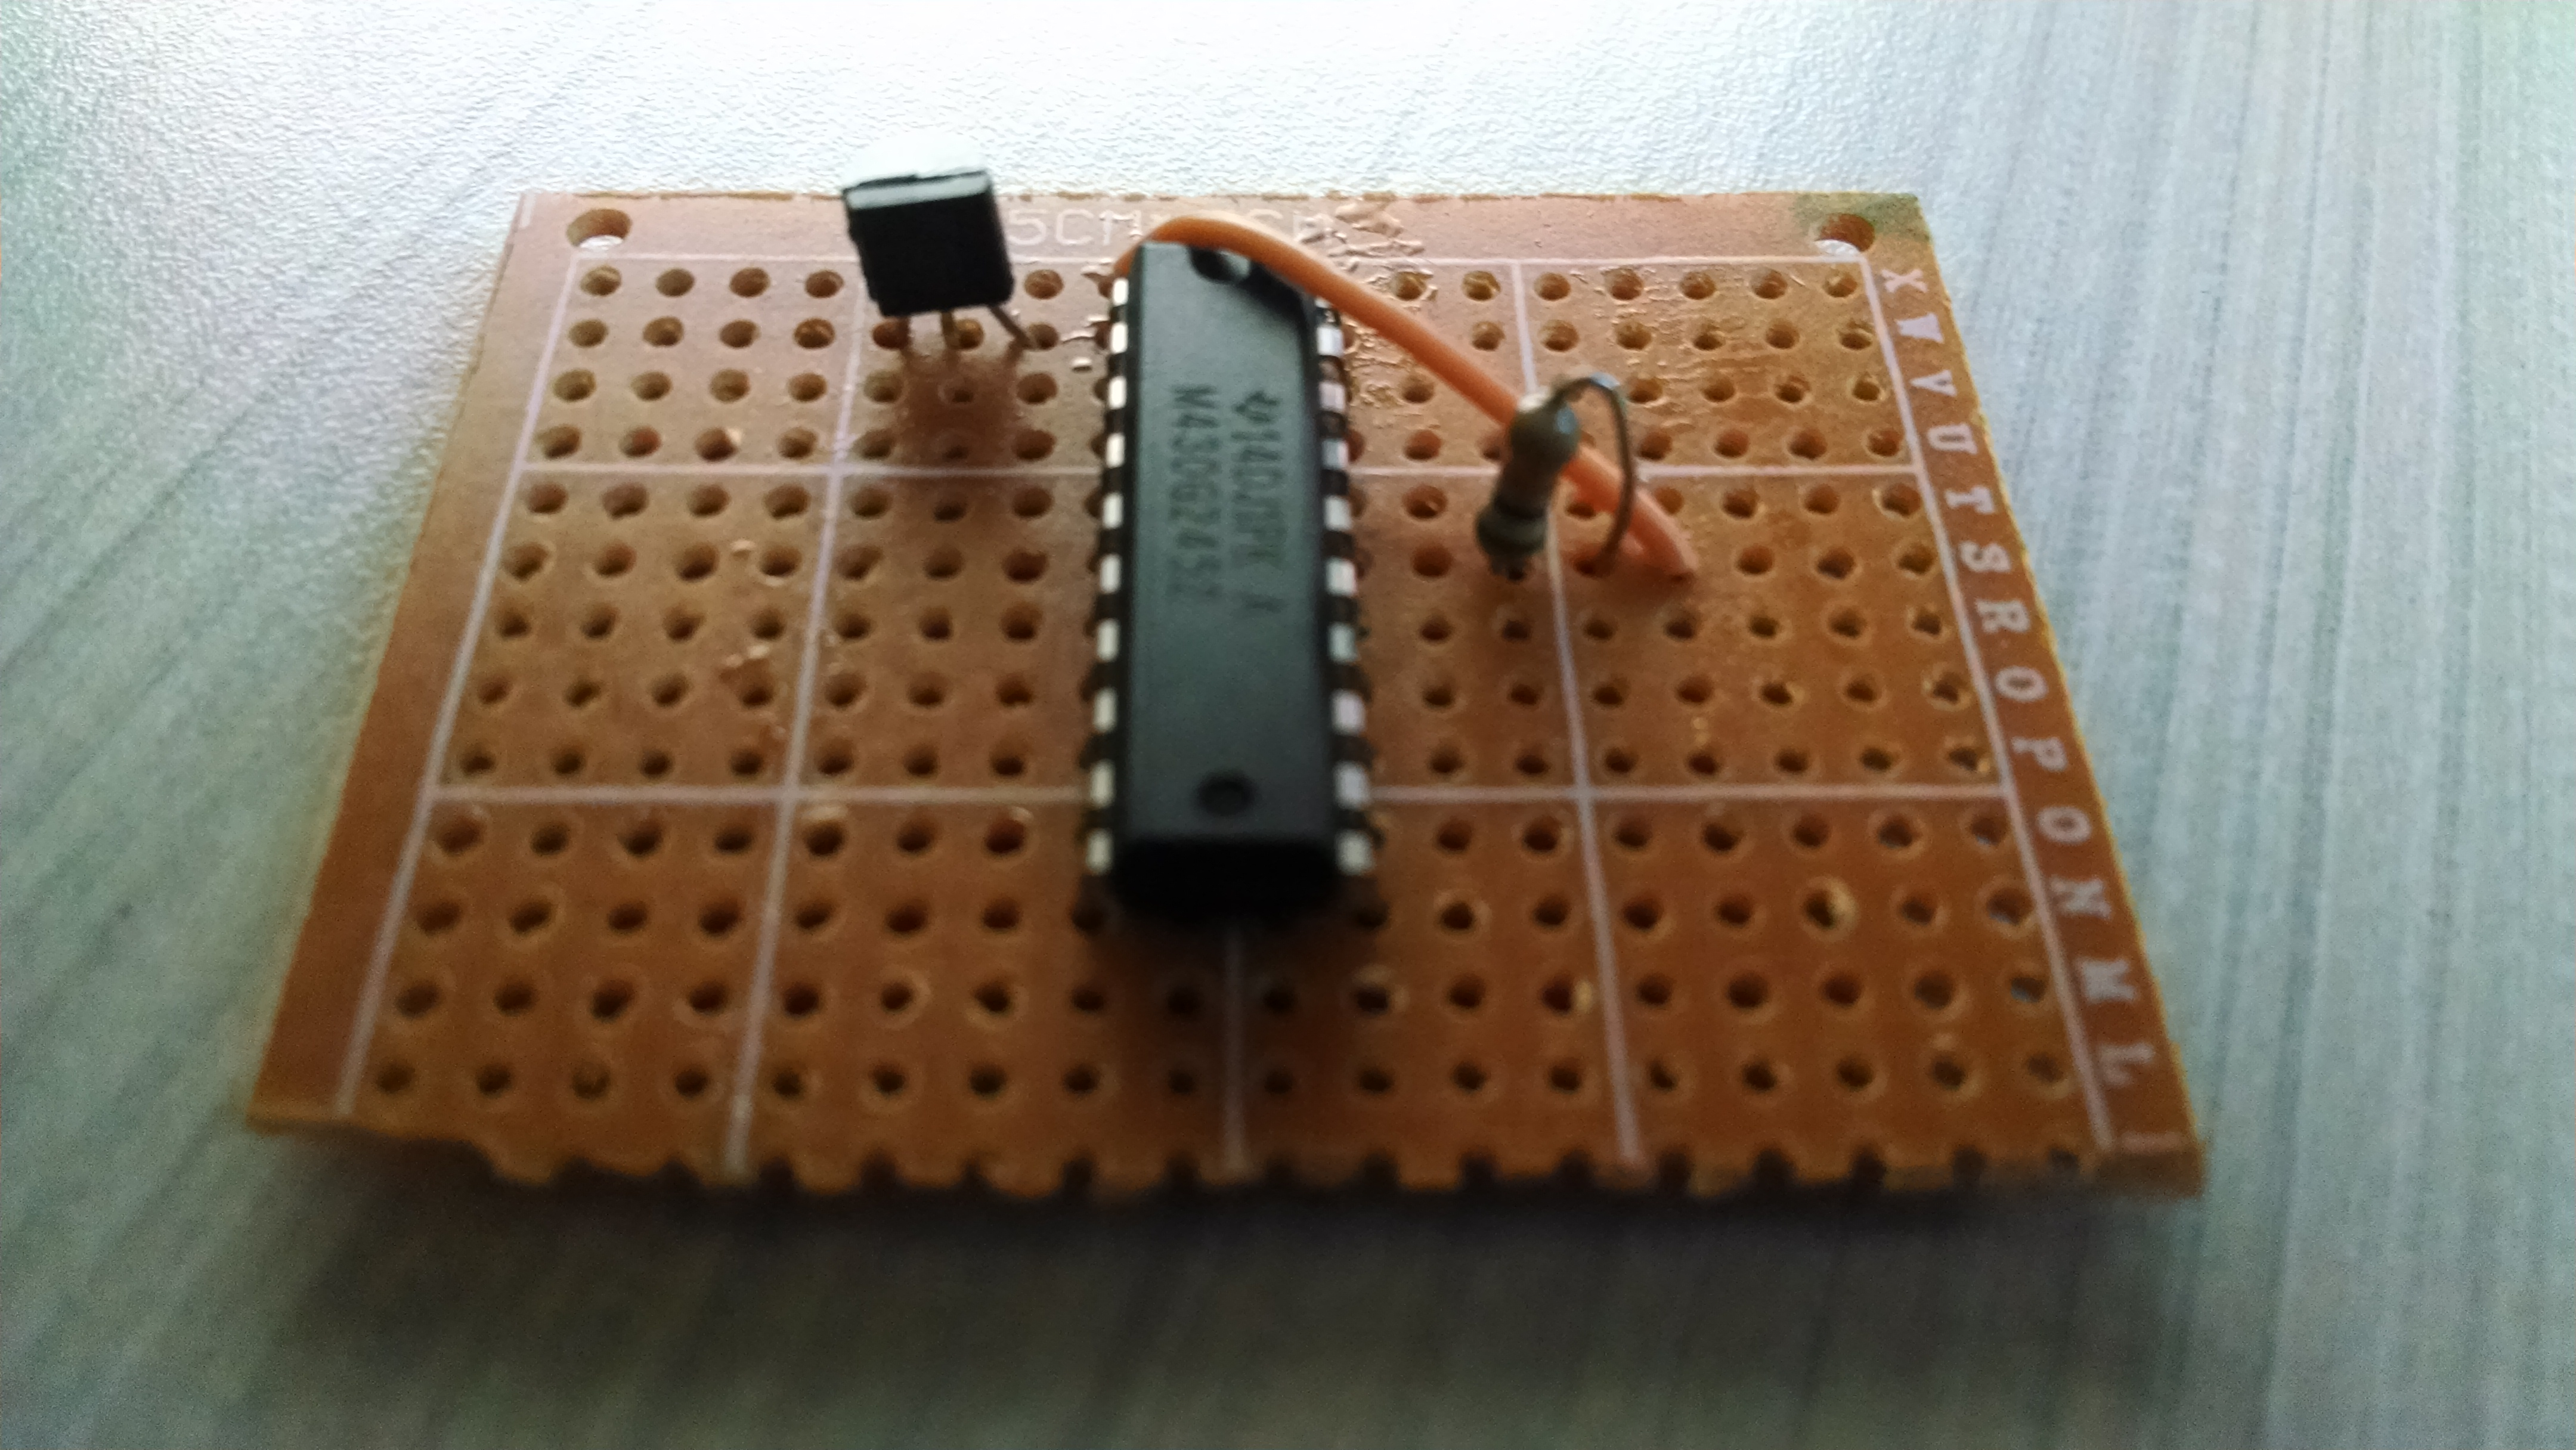
\includegraphics[width=1\textwidth]{board.jpg}
    \caption{One of the development boards without additional parts.}
    \label{fig:board}
\end{figure}

\begin{figure}[p]
    \centering
    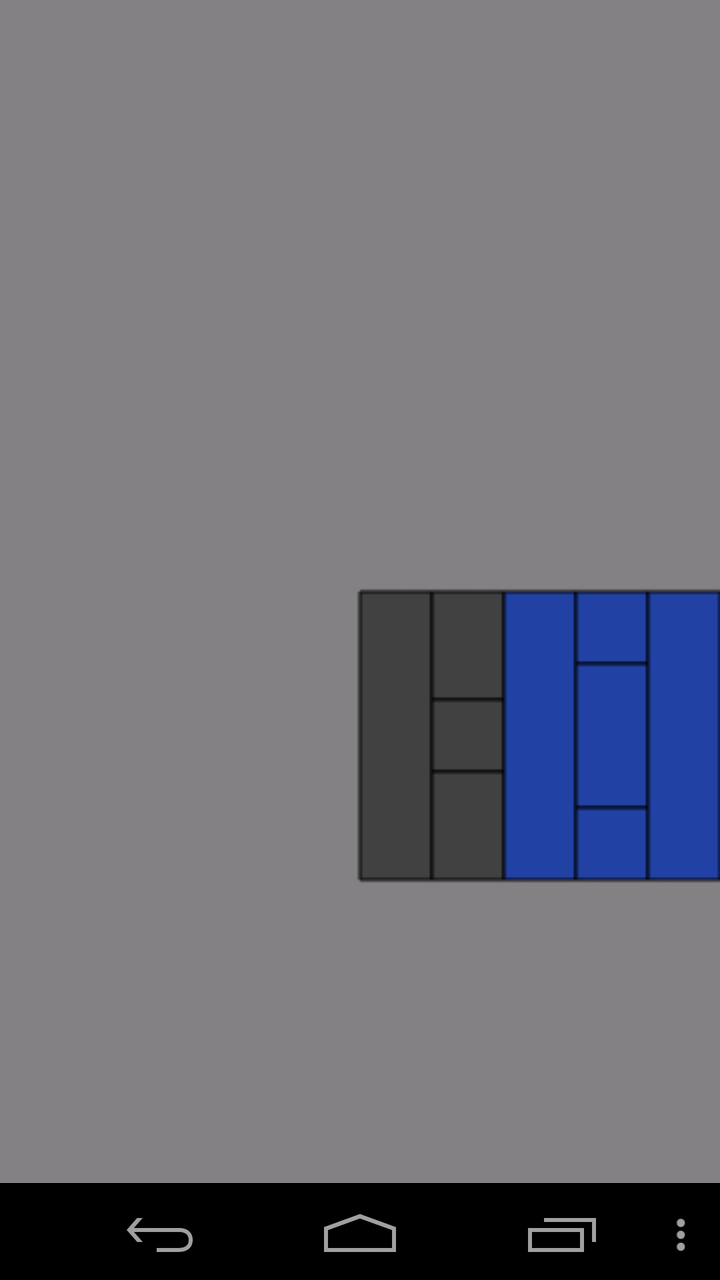
\includegraphics[width=1\textwidth]{prototype.png}
    \caption{Prototyping with Android}
    \label{fig:board}
\end{figure}

\end{document}
